\documentclass[letterpaper,final,12pt,reqno]{amsart}

\usepackage[total={6.3in,9.2in},top=1.1in,left=1.1in]{geometry}

\usepackage{times,bm,bbm,empheq,fancyvrb,graphicx}
\usepackage[dvipsnames]{xcolor}
\usepackage{tikz}
\usetikzlibrary{decorations.pathreplacing}

% hyperref should be the last package we load
\usepackage[pdftex,
colorlinks=true,
plainpages=false, % only if colorlinks=true
linkcolor=blue,   % ...
citecolor=Red,    % ...
urlcolor=black    % ...
]{hyperref}

\renewcommand{\baselinestretch}{1.05}

\newtheorem{lemma}{Lemma}

\newcommand{\Matlab}{\textsc{Matlab}\xspace}
\newcommand{\eps}{\epsilon}
\newcommand{\RR}{\mathbb{R}}

\newcommand{\grad}{\nabla}
\newcommand{\Div}{\nabla\cdot}
\newcommand{\trace}{\operatorname{tr}}

\newcommand{\hbn}{\hat{\mathbf{n}}}

\newcommand{\bg}{\mathbf{g}}
\newcommand{\bn}{\mathbf{n}}
\newcommand{\bu}{\mathbf{u}}
\newcommand{\bv}{\mathbf{v}}
\newcommand{\bx}{\mathbf{x}}

\newcommand{\bV}{\mathbf{V}}
\newcommand{\bX}{\mathbf{X}}

\newcommand{\bxi}{\bm{\xi}}

\newcommand{\bzero}{\bm{0}}

\newcommand{\rhoi}{\rho_{\text{i}}}

\newcommand{\cref}{c_{\text{ref}}}
\newcommand{\Href}{H_{\text{ref}}}
\newcommand{\num}{\nu_{\text{m}}}
\newcommand{\rhom}{\rho_{\text{m}}}


\begin{document}
\title{Evolving glacier geometry using Stokes dynamics}

\author{Ed Bueler}

% Co-author thoughts:
%   * L.~Mitchell because of \texttt{SemiCoarsened...()} etc.~ code (actual)
%   * C.~Khrulev because of implementation and analysis help (prospect)
%   * R.~Sayag because of validation experiment (prospect)
%   * M.~Knepley because of performance help and analysis (prospect)
%   * D.~Shapero because of firedrake help (actual) and implementation or application (prospect)

\maketitle

\thispagestyle{empty}
\bigskip

\section{Introduction} \label{sec:intro}

The most important questions in glaciology concern how the climate around a glacier determines its geometry, both through mass balance and stresses along the ice surface and through internal flow dynamics.  In particular, relationships between surface mass inputs and the geometry of the ice mass are important because they affect sea level, deformations of the Earth's crust, and fresh water supplies, for example.  In this context, evolving-geometry simulations are used by scientists to understand the size and extent of glaciers and ice sheets.  A variety of methodologies for such numerical simulations are seen in practice, with most of the well-established schemes involving shallowness approximations of the continuum equations \cite[for example]{Hoffmanetal2018,Lipscombetal2019,Winkelmannetal2011}.  Furthermore, most methods use explicit or semi-implicit time-stepping \cite{HindmarshPayne1996,Hoffmanetal2018,Lipscombetal2019,Winkelmannetal2011}, with small stability-imposed time steps at high spatial resolution, though fully-implicit exceptions exist \cite{Brinkerhoffetal2017,Bueler2016}.  The performance properties of present-day numerical models therefore limit either the physical modeling authenticity (due to shallowness and other approximations) or the spatial resolution (due to solver performance limitations).  In particular, the quality of ensemble simulations, regarding tradeoffs between the number of ensemble members and the capability of the individual simulations, is directly limited by numerical model performance.

This paper\footnote{version: \today.} addresses an important, but also restricted, class of numerical glacier and ice sheet models which are based on conservation of momentum and mass and which avoid shallowness assumptions.  For conservation of momentum we use the standard shear-thinning (Glen) power-law Stokes model.  Noting that ``mass conservation'' properly refers both to fluid incompressibility and to conservation at the ice surface, we simultaneously solve the stress balance and zero divergence equations for bulk ice \emph{and} the surface kinematical equation (or kinematic boundary condition \cite{GreveBlatter2009}), into which the surface mass balance is a source term.  We model two- and three-dimensional grounded glaciers and ice sheets for which there is a well-defined ice thickness; overhanging ice is not modeled.  Note that the ice thickness is defined at all map-plane points but it is zero in those locations where the (coupled and solved) surface balance and ice flow do not determine the presence of glacier ice.  The solution process determines the glacier extent and the location of the free boundary at the ice margin \cite{SchoofHewitt2013} (Figure \ref{fig:context}).

\begin{figure}[ht]
\begin{center}
\includegraphics[width=0.7\textwidth]{figs/context.pdf}
\end{center}
\caption{We consider 3D models of grounded glaciers and ice sheets which are based on Glen-Stokes ice flow, an evolving free surface, and a free boundary.}
\label{fig:context}
\end{figure}

We do not, however, consider the conservation of energy, and neither thermomechanical coupling nor basal melt are included in our model.  A further restriction is that our ice sticks to the bed (no slip), and we do not consider floating ice.  These restrictions are removable by well-known modeling mechanisms \cite[for example]{Aschwandenetal2012,Winkelmannetal2011}, but how these components affect the performance of fully-coupled implicit time-stepping models like the one here is a topic for further research.

A substantial amount of this paper concerns the time semi-discretized model, wherein each time step solves an inequality-constrained, continuous-space problem.  We will be concerned with, but by no means resolve, the well-posedness of time steps in this model.

Starting in section \ref{sec:finiteelement} we discretize the continuum equations in space with a finite element (FE) method \cite{Elmanetal2014} implemented using the Firedrake library \cite{Rathgeberetal2016} in Python.\footnote{These Python programs are open-source at \href{https://github.com/bueler/stokes-implicit}{\texttt{github.com/bueler/stokes-implicit}}.  FIXME: MAKE REPO PUBLIC.}  We use meshes which are unstructured in the map-plane but which are extruded \cite{Bercea2016,Gibsonetal2019,McRaeetal2016} in the vertical direction.  Mixed elements for velocity, pressure, and vertical ice strain are used, with stable and aspect-ratio robust choices for the velocity-pressure (i.e.~Stokes) block \cite{Elmanetal2014}.  Solutions of the resulting nonlinear discrete equations apply multigrid-preconditioned Newton-Krylov methods \cite{Bueler2021} via PETSc \cite{Balayetal2020}, with semicoarsening in the vertical direction \cite{Tuminaroetal2016}, and all computations are parallelized.

FIXME time-dependent numerical solvers for free surface flows exist outside of glacier applications; approaches like the marker-and-cell method \cite{HarlowWelch1965} make explicit updates to the fluid surface but these are understood to have diffusion-type stability limitations where the maximum time step scales with the square of spatial mesh sizes; we will see this along the way; in such terms our target here is the implementation of very long time steps, e.g.~hundreds to millions of times longer than stable explicit (diffusional) time-steps; indeed we seek the direct computation of steady states as has been demonstrated for the lubrication approximation (SIA) case in \cite{Bueler2016}

FIXME compare literature of existing solvers for glaciers and ice sheets:
\begin{itemize}
\item  nonevolving surface Stokes \cite{IsaacStadlerGhattas2015,Lengetal2013,Lengetal2014a,Zwingeretal2007} (CHECK)
\item  explicitly evolving surface \cite{Gudmundsson1999,HelanowAhlkrona2018,Jouvetetal2008,Larouretal2012,
Lengetal2014b,Lengetal2012,LeysingerGudmundsson2004,PralongFunk2004,Seddiketal2012} (CHECK)
\item significant hydrostatic/B-P \cite{BrownSmithAhmadia2013,Tuminaroetal2016}
\end{itemize}

One model performance metric introduced here is a natural one for glacier modeling.  Namely, we measure the run time of our coupled Glen-Stokes simulations relative to the well-understood computation of ice velocity in the shallow ice approximation (SIA) \cite{Fowler1997} on the same mesh.  That is, we define a glacier model ``work unit'' as the time needed for a diagnostic computation of the SIA horizontal velocity solution.

A primary purpose of this paper is to understand the performance characteristics of numerical simulations using fully-implicit time-stepping with evolving-surface Glen-Stokes models.  At each time step the stress balance, incompressibility, and surface kinematical equations are solved simultaneously to within a tolerance on the coupled residual.  Time steps of order one year are targeted but we identify geometry error metrics may be used to limit and adjust time steps.  To evaluate our approach we validate the model based on results of laboratory experiments, we compare the performance of the model with shallow models, we demonstrate solver optimality and scalability, and we show a solution for the Greenland ice sheet.  At the end we identify spatial resolutions at which the performance of our model would actually exceed that of explicit time-stepping SIA models.


\section{Equations for ice flow in glaciers} \label{sec:strongform}

The standard model for the flow of glaciers uses Stokes equations based upon Glen's shear-thinning flow law for ice \cite{GreveBlatter2009,JouvetRappaz2011,SchoofHewitt2013}.  We will consider this model on time-dependent $d=2,3$ dimensional domains $\Omega^t \subset \RR^d$ (Figure \ref{fig:domainnotation}) for $t>0$ and spatial variables $\bx=(x,y,z)$, with $z$ vertical.  We generally present the equations assuming $d=3$, but in 2D the coordinates are denoted $(x,z)$.

\begin{figure}[ht]
\begin{center}
\includegraphics[width=0.7\textwidth]{figs/domainnotation.pdf}
\end{center}
\caption{Surface mass balance $a$ and bed elevation $b$ are defined on all of the computational domain $R$.  The evolving ice domain $\Omega^t$ has projection $\pi \Omega^t \subset R$.}
\label{fig:domainnotation}
\end{figure}

Allowing any Glen exponent $n\ge 1$, the strong-form equations for bulk ice in $\Omega^t$ are:
\begin{align}
- \nabla \cdot \tau + \nabla p &= \rhoi \bg &&\text{\emph{stress balance}} \label{forcebalance} \\
\nabla \cdot \bu &= 0 &&\text{\emph{incompressibility}} \label{incompressible} \\
\tau &= B_n |D\bu|^{(1/n) - 1} D\bu  &&\text{\emph{flow law}} \label{viscflowlaw}
\end{align}
Solution fields are velocity $\bu$, pressure $p$, and the deviatoric stress tensor $\tau$.  In concrete computational cases later in the paper we use constant ice density $\rhoi=910 \,\text{kg}\,\text{m}^{-3}$ and gravity $\bg=\left<0,0,-g\right>$, with $g=9.81\,\text{m}\,\text{s}^{-2}$.  Note $B_n$ is the $n$-dependent ice hardness, with $n=3$ and $B_n=6.8082\times 10^7\,\text{Pa}\,\text{s}^{1/3}$ \cite{Bueleretal2005} used in computations.

Regarding tensors and their notation, the full (Cauchy) stress tensor $\sigma$ \cite{GreveBlatter2009} decomposes into the deviatoric part $\tau$ minus the pressure, i.e.~$\sigma = \tau - p\,I$, so equation \eqref{forcebalance} simply says $-\Div \sigma = \rhoi \bg$.  The strain rate tensor $D\bu$ is the symmetric part of $\grad \bu$, i.e.~$(D\bu)_{ij} = \frac{1}{2} \left(\grad\bu + \grad\bu^\top\right)$.  Because $D\bu$ is symmetric, and because it has trace zero by equation \eqref{incompressible}, i.e.~$\trace(D\bu)=\nabla \cdot \bu = 0$, from equation \eqref{viscflowlaw} it follows that $\tau$ is also symmetric with trace zero.  The tensor norm in \eqref{viscflowlaw} satisfies $|D\bu|^2 = \frac{1}{2} \trace\left((D\bu)^2\right) = \frac{1}{2} (D\bu)_{ij} (D\bu)_{ij}$.

For the linear Stokes equations \cite{Elmanetal2014}, i.e.~the $n=1$ case, one would traditionally write the flow law \eqref{viscflowlaw} as $\tau = 2\nu D\bu$, and the viscosity would be $\nu = (1/2) B_1$.  For powers $n>1$, namely shear-thinning ice, one defines an ``effective viscosity'' in equation \eqref{viscflowlaw} which involves a negative power of the strain rate norm $|D\bu|$.  This effective viscosity would be singular in the limit of small strain rates, and so, motivated by the expected finite viscosity of glacier ice \cite{GreveBlatter2009}, and noting that the above equations using such a regularization are well-posed for a fixed domain \cite{JouvetRappaz2011}, we define the regularized effective viscosity
\begin{equation}
\nu_\eps(|D\bu|) = \frac{1}{2} B_n \left(|D\bu|^2 + \eps\, D_0^2\right)^{(r-2)/2} \label{regeffvisc}
\end{equation}
where $\eps = 10^{-4}$ and $r=(1/n)+1=4/3$.  The constant $D_0$ defines a strain-rate scale for glacier flow; our value $D_0 = 2 \,\text{a}^{-1}$ corresponds to a velocity difference of 1000 meters per year in a distance of 500 meters.

Using \eqref{regeffvisc} we eliminate $\tau$ from equation \eqref{forcebalance} and rewrite the system in terms of velocity and pressure derivatives only:
\begin{align}
- \nabla \cdot \left(2 \nu_\eps(|D\bu|)\, D\bu\right) + \nabla p &= \rhoi \mathbf{g} \label{stokes} \\
\Div \bu &= 0 \label{incompagain}
\end{align}
The solution to this Glen-Stokes model for bulk ice motion is a velocity-pressure pair $(\bu,p)$, from which one may derive strain rates $D\bu$ and thus stresses $\tau$ and $\sigma$.

Glacier-suitable dynamic boundary conditions will be used, with an emphasis on isolated and grounded ice sheets.  In such cases the ice flow extends in the horizontal direction until a free boundary at the glacier margin is reached.  Real glacier margins may occur as fracture-generated cliffs, but such non-fluid processes are not modeled here.  We assume that the ice thickness is well-defined and thus that the top and bottom boundaries of $\Omega^t$ can, at each time, be identified.  On top we set a condition of zero applied stress,
\begin{align}
\left(2 \nu_\eps(|D\bu|) D\bu - pI\right) \bn &= \bzero  &&\text{\emph{top}: } \overline{\partial} \Omega^t \label{topbc} \\
\intertext{where $\bn$ is normal to the surface.  On the base we require no slip:}
\bu &= \bzero  &&\text{\emph{base}: } \underline{\partial} \Omega^t \label{basebc}
\end{align}
Optionally, to allow simulation of a certain laboratory experiment \cite{SayagWorster2013} (below), we also allow inflow.  Here a prescribed velocity is applied, $\bu = \bu_{\text{in}}$ on an inflow boundary $\partial_{\text{in}} \Omega^t$, subject to $\bu_{\text{in}}\cdot \bn \le 0$ where $\bn$ is an outward normal.

The well-posedness of the above model \eqref{regeffvisc}--\eqref{basebc} is proven by \cite{JouvetRappaz2011}.  Thus if the ice geometry $\Omega^t$ is known then the solution is a unique pair $(\bu,p)$.  Note that the slowness of the fluid, i.e.~zero Reynolds number, implies that at each instant the boundary stresses and body forces determine velocity and pressure fields without any ``memory'' of prior states or influence from inertia, as would occur in the Navier-Stokes equations \cite{Fowler1997}.


\section{Ice geometry evolution} \label{sec:stronggeometry}

The above equations do not describe how a glacier changes shape or extent.  This process, coupled to the flow velocity but not fully determined by it, is described by an additional equation which states conservation of mass on the top boundary $\overline{\partial} \Omega^t$.  To present this equation we first assume a larger map-plane domain $R\subset \RR^{d-1}$ on which the surface mass balance and bedrock elevation data of the problem are defined; again see Figure \ref{fig:domainnotation}.  We will consider only isolated glaciers and ice sheets, so ice must not be present on, nor flow across, the boundary of $R$, and the ice-covered area $\pi\Omega^t$ is a compact subset of $R$.

Let $z=b(x,y)$ be the bedrock elevation, assumed continuously-differentiable and time-independent for simplicity, and $z=h(t,x,y)$ the ice surface elevation; both functions are defined for all $(x,y)\in R$.  The function $h$ is part of the solution while $b$ is input data.  The following form for the time-dependent, open ice domain is assumed:
\begin{equation}
\Omega^t = \left\{\bx\,\big|\,(x,y)\in R \,\text{ and }\, b(x,y) < z < h(t,x,y)\right\}.  \label{Omegat}
\end{equation}
Note that an admissibility requirement for $h$, as a part of the model solution, is that at each $t>0$ and $(x,y)\in R$ we have $h(t,x,y) \ge b(x,y)$.  On the other hand, at any given map-plane location $(x,y)$ the ice may be present (strict inequality) or absent (equality) in an evolving, time-dependent manner.

In agreement with almost all ice sheet and glacier modeling literature, \eqref{Omegat} states that the upper and lower surfaces of the ice mass are described by a well-defined functions of map-plane location.  The domain $\Omega^t$ is thus a layer \cite{Bueler2020}, and not general.  Furthermore we assume a disjoint boundary decomposition $\partial \Omega^t = \overline{\partial} \Omega^t \cup \underline{\partial} \Omega^t$, except for a set of measure zero along the margin.\footnote{An exception to this assertion is for an inflow: $\partial_{\text{in}} \Omega^t \ne \emptyset$.}  Looking ahead, this layer assumption is compatible with our FE method (section \ref{sec:finiteelement}) based on a vertically-extruded, unstructured mesh in the map plane.

Let $a(t,x,y,z)$ be the modeled climatic surface mass balance, in (ice-equivalent) units $\text{m}\,\text{s}^{-1}$.  This scalar field must be defined for all locations above the bedrock elevation, i.e.~$(x,y,z) \in R\times[b(x,y),\infty)$.  Denoting the velocity components as $\bu=\left<u,v,w\right>$, the surface kinematical equation \cite{GreveBlatter2009} then applies on the top of the ice, namely $\frac{\partial h}{\partial t} = a - u \frac{\partial h}{\partial x} - v \frac{\partial h}{\partial y} + w$ or, stated using vector notation,
\begin{equation}
\frac{\partial h}{\partial t} = a + \bu \cdot \bn \quad \text{ on } \overline{\partial}\Omega^t, \label{surfacekinematical}
\end{equation}
where $\bn = \left<-\frac{\partial h}{\partial x},-\frac{\partial h}{\partial y},1\right>$ points upward and is normal to the ice surface.  The surface mass balance $a$ in \eqref{surfacekinematical} is the trace \cite{Evans2010} of the mass balance along the ice surface, i.e.~$a = a(t,x,y,h(t,x,y))$, and similarly for the velocity $\bu = \bu(t,x,y,h(t,x,y))$.  Equation \eqref{surfacekinematical} is often regarded as similar to an advection of $h$, or the ice thickness, but because ice also tends to flow downhill, i.e. generally speaking $\bu \sim -\grad h$, the equation is diffusive at large scale.  Modeled melting or freeze-on at the ice base would add a basal kinematic equation \cite[for example]{Aschwandenetal2012}, but for simplicity this is not considered here.

Equation \eqref{surfacekinematical} applies on the ice surface, that is, where ice is present.  However, the equation should actually be understood as the following problem for the entire computational domain $R$ \cite{SchoofHewitt2013}:
\begin{align}
h-b &\ge 0, \label{strongadmissibility} \\
\frac{\partial h}{\partial t} - a - \bu \cdot \bn &\ge 0, \label{stronginequality} \\
(h-b) \left(\frac{\partial h}{\partial t} - a - \bu \cdot \bn\right) &= 0. \label{strongcomplementarity}
\end{align}
These statements, a nonlinear complementarity problem (NCP) \cite{Bueler2016,Bueler2020,Calvoetal2002}, avoid referring to glacier extent, which we certainly regard as part of the solution.  Equation \eqref{strongcomplementarity}, the complementarity principle, says that either there is no ice at the location ($h=b$) or ice is present and equation \eqref{surfacekinematical} applies.  At ice-free locations, where $\partial h/\partial t=0$ and $\bu=\bzero$, \eqref{stronginequality} says that $a \le 0$, that is, the surface mass balance is not positive.  Physically-speaking, at such locations snow melt and runoff exceed solid precipitation, and ice has not been able to flow there either.

The NCP \eqref{strongadmissibility}--\eqref{strongcomplementarity} can be regarded as having only the time-dependent surface elevation $h$ as the unknown or state vector.  In particular, where $\bu$ appears in the NCP it is the image of a nonlinear and nonlocal map from ice geometry to the surface value of the solution velocity $\bu$, namely by solving \eqref{regeffvisc}--\eqref{basebc}.  That is, the velocity $\bu$ in the surface kinematical equation, whether stated as the classic equation \eqref{surfacekinematical} or through the NCP, can be written as ``$\bu(h)$'' if desired.  (In the current paper, bed elevation $b$ is fixed data.)

Informally, but commonly in the ice sheet modeling literature, the surface kinematical equation determines how the ice surface elevation is updated: the climatically added or removed ice $a\,\Delta t$, plus the component of the ice motion in direction $\bn$, determines the vertical displacement of the surface.  Most numerical glacier models therefore evolve the time-dependent surface $z=h$ by explicit steps, i.e.~$\Delta h \approx \left(a + \bu\cdot \bn\right) \Delta t$ in the simplest forward-Euler case, based upon the current values of $a$, $\bu$, and $\bn$ (i.e.~$\grad h$).  However, for the current paper we will solve \eqref{surfacekinematical}, more precisely \eqref{strongadmissibility}--\eqref{strongcomplementarity}, implicitly and coupled with the Glen-Stokes system \eqref{regeffvisc}--\eqref{basebc}.  The new ice surface will be compatible with the new flow when the solver has converged.

Note that the mass balance $a(t,x,y,z)$ is computed using a separate model for the dynamical state of the atmosphere, one which computes snow precipitation, (atmospheric) energy-driven melt at snow/ice surfaces, and liquid water runoff.  How this is done is well beyond our scope, but it is important in moving-margin glacier simulations that $a$ have a well-defined value both at the current ice surface and elsewhere, or at least nearby.  This is because a simulated glacier can only move into new areas, retreat from ice-covered areas, and undergo changes of surface elevation, if the source term at the new locations is well-defined.  This issue can be ignored for explicit time-steps, but not here.

Appendix A summarizes a simplified model of our coupled problem, namely the shallow ice approximation (SIA), but we will only need this simplification as a source of initial conditions and in performance comparisons.


\section{Time steps and geometry perturbations} \label{sec:perturb}

We intend to solve the coupled problem \eqref{regeffvisc}--\eqref{basebc}, \eqref{strongadmissibility}--\eqref{strongcomplementarity} to yield a triple of functions $\bu,p,h$ where the surface elevation $h$ is defined on $(t,x,y) \in [0,\infty)\times R$.  By \eqref{Omegat}, the solution $h$ defines the domains $\Omega^t\subset \RR^d$ on which the velocity and pressure $\bu,p$ are defined.  However, inequalities \eqref{strongadmissibility} and \eqref{stronginequality} make it clear that we are not solving a true system of coupled PDEs.  In a preliminary manner in this section, then more completely in later sections, we describe function spaces suitable for this inequality-constrained evolving-geometry problem.  In preparation for examining the numerical stability of our implicit time-stepping method (section \ref{sec:implicitstep}), we also attempt to understand how small perturbations of surface elevation would evolve.

\newcommand{\PiK}{\Pi_{\mathcal{K}}}

Let $\mathcal{X}$ be a Banach space of real-valued functions on $R \subset \RR^{d-1}$ containing the bed elevation function $b$.  Let
    $$\mathcal{K} = \{h \in \mathcal{X}\,:\,h \ge b\}$$
be the closed and convex subset of admissible surface elevation functions.  Associated to this set we have a pointwise truncation map $\PiK : \mathcal{X} \to \mathcal{K}$ given by $\PiK f = \max\{b,f\}$.

Because the gradient of $h$ appears in stating our problem---see \eqref{topbc}, \eqref{stronginequality}, \eqref{strongcomplementarity}---we suppose $\mathcal{X}$ is in fact a Sobolev space \cite{Evans2010}, perhaps $W^{1,p}(R)$ for some $p\ge 1$.  While it it is not apparent from the literature which is the correct or natural space $\mathcal{X}$, in the smooth-bed SIA simplified model one would regard it as the space of $n/(2n+2) = 3/8$ powers of functions from $W^{1,n+1}(R)=W^{1,4}(R)$ \cite{JouvetBueler2012}.  In fact, our only requirement in this section for $\mathcal{X}$ is that such functions are continuous, a property satisfied by $W^{1,p}(R)$ if $p>d-1$ \cite[theorem 5.6.5]{Evans2010}.

\newcommand{\hin}{h_{\text{in}}}
\newcommand{\hout}{h_{\text{out}}}

\newcommand{\dhin}{\delta h_{\text{in}}}
\newcommand{\dhout}{\delta h_{\text{out}}}

Fix $h_0 \in \mathcal{K}$ and consider the coupled solution over an increment of time $[t,t+\Delta t]$ starting from this surface elevation.  This solution yields a final surface elevation $h_1 \in \mathcal{K}$ at $t+\Delta t$ (along with $\bu,p$ which are unimportant here).  If one perturbs the initial geometry to $h_0+\dhin$ then a coupled solution generates a different surface elevation $h_1 + \dhout$.  However, because parts of $R$ are not occupied by ice, even small-magnitude surface elevation perturbations are nontrivially constrained by the requirement that the surface be above the bed.  Therefore for $h_0$ and $h_1$ we define spaces of admissible geometry perturbations
    $$\mathcal{K}_i = \left\{\delta h \in \mathcal{X} \,:\, \delta h \ge b - h_i\right\}.$$
Note $h_i+\delta h \in \mathcal{K}$ is equivalent to $\delta h \in \mathcal{K}_i$.

Now consider the exact (coupled) solution process as a nonlinear operator on surface elevation perturbations:
\begin{equation}
\Phi_{a,\Delta t} : \mathcal{K}_0 \to \mathcal{K}_1. \label{perturboperatorexact}
\end{equation}
This map is defined as follows: For $\dhin\in \mathcal{K}_0$ solve the coupled problem \eqref{regeffvisc}--\eqref{basebc}, \eqref{strongadmissibility}--\eqref{strongcomplementarity} using initial geometry $\hin=h_0+\dhin \in \mathcal{K}$ and the generally time-dependent surface mass balance $a$ over $[t,t+\Delta t]\times R$.  This generates $\hout \in \mathcal{K}$; compute $\dhout= \hout - h_1 \in \mathcal{K}_1$.

We seek to compare the action of certain single stage time-stepping schemes to the exact operator in \eqref{perturboperatorexact}.  For this purpose we take the preferred surface mass balance field which may be applied in all such single stage schemes, namely the average
\begin{equation}
\bar a(x,y,z) = \frac{1}{\Delta t} \int_t^{t+\Delta t} a(\tau,x,y,z)\,d\tau.  \label{smbaverage}
\end{equation}
In the rest of the paper we will suppose that the surface mass balance used in solving the coupled problem is held at $\bar a$ over the duration of the time step $[t,t+\Delta t]$.

Existing Stokes solvers for evolving ice sheet geometry \cite{Gudmundsson1999,HelanowAhlkrona2018,Jouvetetal2008,Larouretal2012,
Lengetal2014b,Lengetal2012,LeysingerGudmundsson2004,PralongFunk2004,Seddiketal2012} % CHECK
approximate the exact operator $\Phi_{a,\Delta t}$ in \eqref{perturboperatorexact} by a procedure which amounts to solving for $\bu,p$ first, then applying the explicit approximation of the surface kinematical equation \eqref{surfacekinematical}, and then truncating the resulting surface elevation.  The last step is required because the explicit approximation of \eqref{surfacekinematical}, even when only computed on the current ice surface, may, in places, go below the bed, and indeed this generically happens when the margin retreats.  The stability properties of such explicit solvers is largely unexplored, but it is clear that time steps cannot be arbitrarily large, and that computable estimates of time-step bounds would be useful to practitioners.

To understand such explicit schemes as operators on perturbations comparable to the exact map $\Phi_{a,\Delta t}$, for clarity we present only the forward Euler case.  First we must define the unperturbed result $\hat h_1$ from the scheme.  For this we start from geometry $h_0$, solve only the Stokes problem \eqref{regeffvisc}--\eqref{basebc} to yield $\bu,p$, and use the velocity in the forward Euler approximation of the surface kinematical equation \eqref{surfacekinematical} to compute $\Delta h = \left(a + \bu\cdot \bn\right) \Delta t$.  However, $h_0+\Delta h$ is generally not admissible (in $\mathcal{K}$) so we truncate to get $h^E_1 = \Pi(h_0+\Delta h)$.  This defines a set $\mathcal{K}^E_1$ of admissible output perturbations so we may describe the map on perturbations as
\begin{equation}
\Phi^E_{\bar a,\Delta t} : \mathcal{K}_0 \to \mathcal{K}^E_1. \label{perturboperatorexplicit}
\end{equation}
It is computed by the following steps.  From $\dhin\in \mathcal{K}_0$ let $\hin=h_0+\dhin$ determine the ice geometry and solve only the Stokes problem \eqref{regeffvisc}--\eqref{basebc} to yield $\bu,p$.  Use the velocity $\bu$ in the forward Euler approximation of the surface kinematical equation \eqref{surfacekinematical} to update the surface, but then truncate to get an admissible geometry, and then subtract to get the admissible output perturbation:
    $$\Phi^E_{\bar a,\Delta t}(\dhin) = \PiK\Big(\hin + \left(\bar a + \bu_{[\hin]} \cdot \bn_{[\hin]}\right) \Delta t\Big) - h^E_1.$$
As a summary heuristic, the action of such an explicit scheme on geometry perturbations is
    $$\Phi^E_{\bar a,\Delta t} = (\text{solve Stokes} \to \text{update surface} \to \text{truncate to geometry}).$$

Compare the action of an implicit time-step scheme, here backward Euler for simplicity.  FIXME
\begin{equation}
\Phi^I_{\bar a,\Delta t} : \mathcal{K}_0 \to \mathcal{K}^I_1. \label{perturboperatorimplicit}
\end{equation}

FIXME note that the three $\Phi$ do not even have the same output spaces [FIXME: MAYBE FORCE THEM TO FOR THE ANALYSIS?], but still we expect both $\Phi^E_{\bar a,\Delta t} = \Phi_{\bar a,\Delta t} + O(\Delta t^1)$ and similarly for $\Phi^I$; but the ops are really different; for the linear heat equation $u_t=Lu$ on a bounded domain we have $\Phi_{\Delta t} = e^{\Delta t\,L}$, $\Phi^E_{\Delta t} = I + \Delta t\,L$, $\Phi^I_{\Delta t} = (I - \Delta t\,L)^{-1}$; here $\Phi^E$ is unbounded while $\Phi$, $\Phi^I$ are bounded and actually compact (send bounded sets to compact, thus nearly finite-dimensional, sets); we expect for the ice problem that $\Phi^E_{\bar a,\Delta t}$ generates large magnitude perturbations for some norm one inputs while $\Phi^I_{\bar a,\Delta t}$ (and the exact) are compact in the same sense as in the linear case

FIXME positive $\delta h$ always allowed; small positive $\delta h$ with small support cause change in velocity field equivalent to the addition of a Stokeslet (if single hump $/\backslash$) or doublet (if $/\backslash/$ with zero added volume) \cite{ChwangWu1975}; the former is longer range and the latter short


\section{Implicit time-stepping via a domain mapping} \label{sec:implicitstep}

Our main purpose is to demonstrate an effective implicit scheme to simultaneously solve the evolving geometry problem \eqref{regeffvisc}--\eqref{basebc}, \eqref{strongadmissibility}--\eqref{strongcomplementarity}.  The only time derivative in this coupled problem appears in the surface kinematical expression, i.e.~in \eqref{stronginequality} and \eqref{strongcomplementarity}.  Because the remaining equations and boundary conditions lack time derivatives, but they apply at all times, the coupled problem should be understood as an infinite-dimensional differential algebraic equation (DAE) problem \cite{AscherPetzold1998}, but with added inequality constraints.

In this section, using a discrete-time and continuous-space formulation, we state our scheme for solving this problem.  A new feature is that at each time step we compute a vertical-only displacement field which captures the effect of the surface kinematical equation along the boundary but which is defined everywhere within the same (reference) domain as the velocity and pressure.  The coupled solution, once found, includes this vertical displacement which then determines the new domain of ice at the end of the time step.

We discretize the coupled problem in time using the first-order backward Euler method.  Higher-order implicit schemes exist, including stiff-decay backward-differentiation schemes \cite{AscherPetzold1998,Bueler2021} suitable for DAE problems.  However, because of the inequality constraints, the numerical errors associated to determining the free boundary are unavoidably of low order in time and space \cite{Bueler2020} and tend to dominate over time-stepping errors made in well-behaved locations.  Effective application of higher-order time-stepping is thus a topic for future research.

The fundamental issue faced by implicit time-stepping schemes for glaciers is that the map-plane region covered by ice will change during the time step.  Either in terms of the 3D, ice-occupied continuum domain $\Omega^t$ of the coupled PDE problem, or in terms of the numerical 3D mesh (section \ref{sec:finiteelement}), one can only solve for ice velocity and pressure in locations where ice or mesh exists.  Concretely, supposing $t_{n-1}$ and $t_n$ are consecutive times with step $\Delta t = t_n - t_{n-1} > 0$, the possibility of glacier advance and retreat during an implicit step requires the PDE domain to cover the current ice at $t_{n-1}$, and locations where ice is present once we have solved the equations at the new time $t_n$.

\begin{figure}[ht]
\begin{center}
\includegraphics[width=0.65\textwidth]{figs/currenttime.pdf}
\vspace{-6mm}

\includegraphics[width=0.65\textwidth]{figs/referencedomain.pdf}
\vspace{-1mm}

\includegraphics[width=0.65\textwidth]{figs/nexttime.pdf}
\end{center}
\caption{The current ice domain $\Omega^{n-1}$ is used to construct a reference domain $\Lambda$.  The coupled solution on $\Lambda$ generates a map from $\Lambda$ to the new domain $\Omega^n$.}
\label{fig:domainupdate}
\end{figure}

Our scheme uses the current ice geometry to construct a reference domain on which the new velocity, pressure, and vertical displacement are found as the coupled problem is solved.  The detailed construction of the reference domain, given next, is not as important as the main idea that the coupled PDE solution must occur on a domain supporting the new ice geometry.  Elimination or creation of ice in any map-plane location must be allowed, so changes in the map-plane topology, as a glacier disconnects for example, must also be allowed.

Let $\Href>0$ be a reference glacier thickness, a value such that grounded ice of uniform thickness $\Href$ flows slowly over the bedrock topography, and which is small compared to observed glacier thicknesses.  For example, $\Href=50$ m might be appropriate for small mountain glaciers while for large, cold, and low-angle ice sheets we might even choose $\Href=500$ m.  (Recall that the velocity of Glen $n=3$ ice in a slab-on-slope geometry \cite{GreveBlatter2009} goes as the $4$th power of the ice thickness, and thus $50$ m ice flows $10^4$ times slower than $500$ m ice.)

Suppose $h^{n-1}(x,y) \approx h(t_{n-1},x,y)$ is an admissible current surface elevation.  Denote the corresponding ice domain by $\Omega^{n-1}=\{\bx\,\big|\,(x,y)\in R, b(x,y)<z<h^{n-1}(x,y)\} \subset \RR^3$; see \eqref{Omegat} and the top of Figure \ref{fig:domainupdate}.  The reference domain will have thickness which is everywhere at least $\Href$, so for $(x,y) \in R$ let
\begin{equation}
\lambda(x,y) = b(x,y) + \max\{\Href,h^{n-1}(x,y)-b(x,y)\}. \label{definelambda}
\end{equation}
The reference domain has surface $z=\lambda(x,y)$:
\begin{equation}
\Lambda = \left\{(\xi,\eta,\zeta)\,\big|\,(\xi,\eta)\in R, \, b(\xi,\eta) < \zeta < \lambda(\xi,\eta)\right\};  \label{Lambda}
\end{equation}
see Figure \ref{fig:domainupdate}.  Observe that $\Omega^{n-1} \subset \Lambda$ and $h^{n-1} \le \lambda$, and that $\Lambda$ and $\lambda$ are fully determined by data which is known at the start of the time step.
% FIXME: COULD INSTEAD MAKE $\lambda$ SMOOTH

From now on $\bxi=(\xi,\eta,\zeta)$ will denote coordinates on $\Lambda \subset \RR^3$.  We will compute the updated domain $\Omega^n \subset \RR^3$ via a change of coordinates, a map
\begin{equation}
\bx(\bxi) = \bxi + (0,0,c(\bxi)) \label{changecoords}
\end{equation}
with nontrivial $z$ coordinate.  This map is based on a new scalar function $c(\bxi)$ which is defined on $\Lambda$ and satisfies certain properties.  One of these is that
\begin{equation}
c(\xi,\eta,b(\xi,\eta))=0, \label{mapbasetobase}
\end{equation}
thus the map preserves the elevation of the bedrock.

The domain $\Omega^n$ is defined to be the interior of the image of $\Lambda$ under map \eqref{changecoords}:
\begin{equation}
\Omega^n = \{\bx(\bxi) \,\big|\, \bxi \in \Lambda\}^\circ. \label{updateddomain}
\end{equation}
Determining $c(\bxi)$ on $\Lambda$ will therefore determine the new ice domain $\Omega^n$.  Since $c(\bxi)$ will solve an elliptic PDE (below), the map is smooth from $\Lambda$ to $\Omega^n$, but it is degenerate.  Its inverse is not generally smooth or even well-defined.  In particular, applying the topological interior in \eqref{updateddomain} is necessary because the map will collapse ice-free locations to zero height, which are then outside $\Omega^n$.  (Here ``ice--free'' refers to the solution geometry.)

Suppose that map \eqref{changecoords} is monotonic in each column, that is, that for each fixed $(\xi,\eta)\in R$ the map takes the interval $I=(b(\xi,\eta),\lambda(\xi,\eta))$ monotonically to a new interval.  This includes the possibility that $I$ is mapped to a single point.  The computed surface elevation $h(\xi,\eta)\approx h(t_n,\xi,\eta)$, including the upper boundary of $\Omega^n$, is defined on all of $R$.  Its value is defined to be the maximum mapped $z$ coordinate in each column:
\begin{equation}
h(\xi,\eta) = \lambda(\xi,\eta) + c(\xi,\eta,\lambda(\xi,\eta)). \label{maptoptotop}
\end{equation}
Thus the top of the reference domain is sent to the top of the new ice domain.  Furthermore, because the map will also be differentiable, it follows from \eqref{mapbasetobase}, \eqref{maptoptotop}, monotonicity, and the requirement that $h$ be admissible ($h\ge b$) that
\begin{equation}
1 + \frac{\partial c}{\partial \zeta}(\bxi) = \frac{\partial z}{\partial \zeta}(\bxi) \ge 0. \label{mapmonotonic}
\end{equation}
That is, the map is a nondecreasing function in each column.  (Though $c$ can have negative values, $z(\lambda) \ge z(b)$ always.)  In locations which are computed to be ice free we have
\begin{equation}
h(\xi,\eta)=b(\xi,\eta) = \zeta + c(\xi,\eta,\zeta) \text{ for all } \zeta \in I, \label{mapcrushes}
\end{equation}
that is, map \eqref{changecoords} sends the entire column to the bed elevation; $c$ is then fully-determined by a linear formula: $c(\xi,\eta,\zeta) = b(\xi,\eta) - \zeta$.  Possibilities are shown in Figure \ref{fig:mapI}.

\begin{figure}[ht]
\begin{tikzpicture}[scale=2.5,font=\small]
\newcommand{\ILABEL}{}
\newcommand{\MIDLABEL}{}
\tikzstyle{grayarrow} = [thick,gray,->,shorten <=7,shorten >=12]

\node[anchor=west] at (0.0,1.7) {\underline{$h \ge \lambda$}:};
\pgfmathsetmacro{\IX}{0.0}
\pgfmathsetmacro{\IY}{1.0}
\renewcommand{\MIDLABEL}{$\lambda$}
% "function" to draw vertical interval with caps
% inputs: \IX = x position
%         \IY = y position of top
%         \ILABEL = text to put below
%         \MIDLABEL = text to put just left of middle of interval
%         \TOPLABEL = text to put just left of top of interval

\draw[thick] (\IX,0.0) node[left] {$b$} -- node[left] {\MIDLABEL} (\IX,\IY) node[left] {\TOPLABEL};
\draw[thick] (\IX-0.05,0.0) -- (\IX+0.05,0.0);
\draw[thick] (\IX-0.05,\IY) -- (\IX+0.05,\IY);
\node at (\IX,-0.2) {\ILABEL};


\pgfmathsetmacro{\IX}{1.0}
\pgfmathsetmacro{\IY}{1.5}
\renewcommand{\MIDLABEL}{$h$}
% "function" to draw vertical interval with caps
% inputs: \IX = x position
%         \IY = y position of top
%         \ILABEL = text to put below
%         \MIDLABEL = text to put just left of middle of interval
%         \TOPLABEL = text to put just left of top of interval

\draw[thick] (\IX,0.0) node[left] {$b$} -- node[left] {\MIDLABEL} (\IX,\IY) node[left] {\TOPLABEL};
\draw[thick] (\IX-0.05,0.0) -- (\IX+0.05,0.0);
\draw[thick] (\IX-0.05,\IY) -- (\IX+0.05,\IY);
\node at (\IX,-0.2) {\ILABEL};


\draw[decoration={brace,mirror,raise=7pt},decorate] (1.0,1.0) -- node[right=7pt] {$c\ge 0$} (1.0,1.5);
\draw[style=grayarrow] (0.0,0.0) -- (1.0,0.0);
\draw[style=grayarrow] (0.0,1.0) -- (1.0,1.5);

\node[anchor=west] at (2.0,1.7) {\underline{$b < h < \lambda$}:};
\pgfmathsetmacro{\IX}{2.0}
\pgfmathsetmacro{\IY}{1.0}
\renewcommand{\MIDLABEL}{$\lambda$}
% "function" to draw vertical interval with caps
% inputs: \IX = x position
%         \IY = y position of top
%         \ILABEL = text to put below
%         \MIDLABEL = text to put just left of middle of interval
%         \TOPLABEL = text to put just left of top of interval

\draw[thick] (\IX,0.0) node[left] {$b$} -- node[left] {\MIDLABEL} (\IX,\IY) node[left] {\TOPLABEL};
\draw[thick] (\IX-0.05,0.0) -- (\IX+0.05,0.0);
\draw[thick] (\IX-0.05,\IY) -- (\IX+0.05,\IY);
\node at (\IX,-0.2) {\ILABEL};


\pgfmathsetmacro{\IX}{3.0}
\pgfmathsetmacro{\IY}{0.5}
\renewcommand{\MIDLABEL}{$h$}
% "function" to draw vertical interval with caps
% inputs: \IX = x position
%         \IY = y position of top
%         \ILABEL = text to put below
%         \MIDLABEL = text to put just left of middle of interval
%         \TOPLABEL = text to put just left of top of interval

\draw[thick] (\IX,0.0) node[left] {$b$} -- node[left] {\MIDLABEL} (\IX,\IY) node[left] {\TOPLABEL};
\draw[thick] (\IX-0.05,0.0) -- (\IX+0.05,0.0);
\draw[thick] (\IX-0.05,\IY) -- (\IX+0.05,\IY);
\node at (\IX,-0.2) {\ILABEL};


\draw[decoration={brace,raise=7pt},decorate] (3.0,1.0) -- node[right=7pt] {$c<0$} (3.0,0.5);
\draw[style=grayarrow] (2.0,0.0) -- (3.0,0.0);
\draw[style=grayarrow] (2.0,1.0) -- (3.0,0.5);

\node[anchor=west] at (4.0,1.7) {\underline{$h=b$}:};
\pgfmathsetmacro{\IX}{4.0}
\pgfmathsetmacro{\IY}{1.0}
\renewcommand{\MIDLABEL}{$\lambda$}
% "function" to draw vertical interval with caps
% inputs: \IX = x position
%         \IY = y position of top
%         \ILABEL = text to put below
%         \MIDLABEL = text to put just left of middle of interval
%         \TOPLABEL = text to put just left of top of interval

\draw[thick] (\IX,0.0) node[left] {$b$} -- node[left] {\MIDLABEL} (\IX,\IY) node[left] {\TOPLABEL};
\draw[thick] (\IX-0.05,0.0) -- (\IX+0.05,0.0);
\draw[thick] (\IX-0.05,\IY) -- (\IX+0.05,\IY);
\node at (\IX,-0.2) {\ILABEL};


\pgfmathsetmacro{\IX}{5.0}
\pgfmathsetmacro{\IY}{0.0}
\renewcommand{\MIDLABEL}{}
% "function" to draw vertical interval with caps
% inputs: \IX = x position
%         \IY = y position of top
%         \ILABEL = text to put below
%         \MIDLABEL = text to put just left of middle of interval
%         \TOPLABEL = text to put just left of top of interval

\draw[thick] (\IX,0.0) node[left] {$b$} -- node[left] {\MIDLABEL} (\IX,\IY) node[left] {\TOPLABEL};
\draw[thick] (\IX-0.05,0.0) -- (\IX+0.05,0.0);
\draw[thick] (\IX-0.05,\IY) -- (\IX+0.05,\IY);
\node at (\IX,-0.2) {\ILABEL};


\draw[decoration={brace,raise=7pt},decorate] (5.0,1.0) -- node[right=7pt] {$c=b-\lambda$} (5.0,0.0);
\draw[style=grayarrow] (4.0,0.0) -- (5.0,0.0);
\draw[style=grayarrow] (4.0,1.0) -- (5.0,0.0);

\end{tikzpicture}


\caption{The map $\bx:\Lambda \to \Omega^n$ in \eqref{changecoords} takes a column with surface elevation $\lambda$ to one of elevation $h$.  The column can grow (left), shrink (middle), or yield no ice (right) according to the top boundary value $c=c(\xi,\eta,\lambda(\xi,\eta))$ from \eqref{claplacetop}.}
\label{fig:mapI}
\end{figure}

On the other hand, our purpose is to approximate the surface kinematical equation \eqref{surfacekinematical} with a backward Euler step.  We intend to solve this equation (among others) in the coupled system on $\Lambda$.  Where there is ice \emph{in the solution} we want the discretized form of \eqref{surfacekinematical} to apply:
\begin{equation}
h(\xi,\eta)>b(\xi,\eta) \quad \iff \quad h - h^{n-1} = \Delta t\left(a + \bu \cdot \bn\right). \label{backwardeulerske}
\end{equation}
The quantities in the right-hand equation are evaluated at the \emph{solution} ice surface $\zeta=h(\xi,\eta)$, i.e.~on the top boundary of $\Omega^n$ at the new time $t_n$.  By \eqref{maptoptotop} the quantities $h$ and $\bn$, in particular, depend on the value $c(\xi,\eta,\lambda(\xi,\eta))$ of $c$ on the top surface of $\Lambda$.  As we are actually seeking to solve NCP \eqref{strongadmissibility}--\eqref{strongcomplementarity}, we emphasize that \eqref{backwardeulerske} applies only where ice is present in the solution geometry.

We now have multiple requirements on the scalar function $c(\bxi)$, specifically equations \eqref{mapbasetobase}, \eqref{mapmonotonic}, \eqref{mapcrushes}, and \eqref{backwardeulerske}.  It is not clear that these requirements can all be satisfied.  The resulting function $c$ will, at least, have low regularity along the boundary of $\Lambda$ because, as one passes from an ice-free location \eqref{mapcrushes} to one with ice \eqref{backwardeulerske}, i.e.~across an ice margin, we should expect $c$ to change abruptly.

Our plan is to compute a well-defined function $c$ which satisfies the given requirements \eqref{mapbasetobase} and \eqref{backwardeulerske} along the boundary $\partial \Lambda$.  Furthermore this function will be smooth within the domain $\Lambda$.  However, within the domain we sacrifice conditions \eqref{mapmonotonic} and \eqref{mapcrushes}.  In locations where the solution has no ice, on the top boundary of $\Lambda$ we do set the value given by \eqref{mapcrushes}: $c=b-\lambda$.  Also, by substituting \eqref{maptoptotop} into \eqref{backwardeulerske}, in locations where the solution has ice, $c=h^{n-1} + \Delta t\left(a + \bu \cdot \bn\right) - \lambda$ will hold on the top boundary; observe that $c$ appears on both sides of this equation.

That is, in our scheme the vertical displacement $c(\bxi)$ solves a coupled Laplace equation boundary value problem on $\Lambda$:
\begin{align}
        \grad^2 c &= 0 &&\text{in } \Lambda \label{claplace} \\
                c &= b\, \mathbbm{1}_{\{h=b\}} + \left(h^{n-1} + \Delta t\left(a + \bu \cdot \bn\right)\right)\, \mathbbm{1}_{\{h>b\}} - \lambda &&\text{top: } \overline{\partial} \Lambda  \label{claplacetop} \\
                c &= 0 &&\text{base: } \underline{\partial} \Lambda,  \label{claplacebase} \\
 \grad c\cdot \bn &= 0 &&\text{sides: } \partial_{|} \Lambda.  \label{claplacesides}
\end{align}
In the top boundary condition \eqref{claplacetop} we use $\mathbbm{1}_S$ as the indicator function of a subset $S\subset \overline{\partial} \Lambda$.  The vertical sides of $\Lambda$, above $\partial R$, are denoted $\partial_{|} \Lambda$.  The Neumann boundary condition on these sides removes influences from outside of the computational domain.  Figure \ref{fig:claplaceproblem} sketches this problem.

\begin{figure}[ht]
\begin{center}
\includegraphics[width=0.85\textwidth]{figs/claplaceproblem.pdf}
\end{center}
\caption{A sketch of reference domain $\Lambda$ and problem \eqref{claplace}--\eqref{claplacesides}.  See the text regarding the top boundary condition \eqref{claplacetop}.}
\label{fig:claplaceproblem}
\end{figure}

The value of ``$h$'' in the top boundary condition \eqref{claplacetop} is the new (solution) surface elevation, that is, the elevation of the top of the ice domain \emph{after} applying the map $\bxi\mapsto \bx$.  This value depends on $c$ through the definition \eqref{maptoptotop}, and in fact \eqref{claplacetop} is a generalization of a Robin boundary condition in this Laplace problem.  However, as one passes across the margin onto the glacier the \eqref{claplacetop} value changes discontinuously from its value given by \eqref{mapcrushes}, i.e.~$c=b-\lambda$, to the generalized-Robin condition \eqref{backwardeulerske}.  Looking ahead, condition \eqref{claplacetop} will be included into the coupled system as a boundary integral term in a mixed-space weak form (see section \ref{sec:finiteelement}).

In the $h>b$ case the quantities $a,\bu,\bn$ in \eqref{claplacetop} are evaluated along the top of $\Lambda$, i.e.~at $\zeta=\lambda(\xi,\eta)$, but these locations are mapped using $c$ to the surface of the solution ice, i.e.~the top boundary of $\Omega^n$.  In particular, as already noted, $\bn$ in \eqref{claplacetop} is the outward normal to $\Omega^n$, not $\Lambda$.  To evaluate $\bn=\left<-\frac{\partial h}{\partial\xi},-\frac{\partial h}{\partial\eta},1\right>$ we compute the two-dimensional gradient $\grad h$; applying the chain rule to \eqref{maptoptotop} reveals
\begin{equation}
\grad h = \left<\frac{\partial c}{\partial\xi},\frac{\partial c}{\partial\eta}\right> + \left(1+\frac{\partial c}{\partial\zeta}\right) \left<\frac{\partial \lambda}{\partial\xi},\frac{\partial \lambda}{\partial\eta}\right>. \label{hgradient}
\end{equation}
Thus in the $h>b$ case \eqref{claplacetop} says
\begin{equation}
c = \phi + \Delta t\,\left(- u\frac{\partial c}{\partial\xi} - v\frac{\partial c}{\partial\eta} + w\right) - \Delta t\,\left(1+\frac{\partial c}{\partial\zeta}\right)\left(u\frac{\partial \lambda}{\partial\xi} + v\frac{\partial \lambda}{\partial\eta}\right), \label{mappednormaldirection}
\end{equation}
where we denote denoting $\bu=\left<u,v,w\right>$.  The uninteresting part $\phi=h^{n-1} + \Delta t\,a - \lambda$ is expected to be at least continuous.

In contrast to \eqref{mappednormaldirection}, a true Robin condition along $\overline{\partial} \Lambda$ would be $c=\beta-\alpha\,\grad c \cdot \bn_{\Lambda}$ for some positive function $\alpha>0$ \cite[p.~154]{Ockendonetal2003}, $\beta$ of either sign, and outward unit normal $\bn_{\Lambda}$.  Expanded using $\bn_{\Lambda} = \left<-\frac{\partial \lambda}{\partial\xi},-\frac{\partial \lambda}{\partial\eta},1\right>$ this says
\begin{equation*}
c=\beta - \alpha\,\left(-\frac{\partial \lambda}{\partial\xi}\frac{\partial c}{\partial\xi} -\frac{\partial \lambda}{\partial\eta}\frac{\partial c}{\partial\eta} + \frac{\partial c}{\partial\zeta}\right).
\end{equation*}
The actual condition \eqref{mappednormaldirection} is thus problematical for two reasons.  First, the directional derivative is not normal to $\partial\Lambda$, and indeed it depends on the direction of the ice velocity $\bu$ (which goes either way across the surface), and an integration by parts will not eliminate the derivatives of $c$ from the statement.  Secondly, $\lambda$ itself, defined in \eqref{definelambda}, will generally have low regularity.

Intuitively, solving problem \eqref{claplace}--\eqref{claplacesides} yields a smooth 3D function $c$ which, in each vertical column of $\Lambda$, connects either the surface kinematical quantity \eqref{backwardeulerske} or the ice-free case \eqref{mapcrushes} as linearly as possible to zero at the base.  Mathematically, $c$ satisfies the maximum principle in $\Lambda$ \cite{Evans2010}, and the direction of $\grad c$ changes direction as little as possible (in the energy norm) while smoothly meeting the boundary data.

The weak form of the coupled problem, stated in the next section, will require derivatives of coordinate transformation \eqref{changecoords}.  The Jacobian is
\begin{equation}
J(\bxi) = \frac{\partial \bx}{\partial \bm{\xi}} = \begin{pmatrix} 1 & 0 & 0 \\ \strut 0 & 1 & 0 \\ \strut \frac{\partial c}{\partial \xi} & \frac{\partial c}{\partial \eta} & 1+\frac{\partial c}{\partial \zeta} \end{pmatrix}, \label{changejac}
\end{equation}
with determinant $\det(J) = 1+\frac{\partial c}{\partial \zeta}$.  For a generic, smooth function $f(\bx)$ defined on $\Omega^n$ the transformation defines $\tilde f(\bxi) = f(\bx(\bxi))$ on $\Lambda$ with gradient $\grad_{\bxi} \tilde f = J^\top \grad_{\bx} f$.  Thus
\begin{equation}
\grad_{\bx} f = (J^\top)^{-1} \grad_{\bxi} \tilde f = \begin{pmatrix} \strut 1 & 0 & - \frac{\partial c}{\partial \xi} \hat\ell \\ \strut 0 & 1 & -\frac{\partial c}{\partial \eta} \hat\ell \\ \strut 0 & 0 & \hat\ell \end{pmatrix} \grad_{\bxi} \tilde f. \label{changegrad}
\end{equation}
where $\hat\ell(\bxi) = \left(1+\frac{\partial c}{\partial \zeta}\right)^{-1}=\det(J)^{-1}$.

Regarding derivatives of vector fields, it follows from \eqref{changegrad} that for $\tilde \bu(\bxi) = \bu(\bx(\bxi)) = \left<\tilde u,\tilde v, \tilde w\right>$ we have
\begin{equation}
\grad_{\bx} \cdot \bu = \grad_{\bxi} \cdot \tilde\bu - \hat\ell \left(\frac{\partial c}{\partial \xi} \frac{\partial \tilde u}{\partial \zeta} + \frac{\partial c}{\partial \eta} \frac{\partial \tilde v}{\partial \zeta}\right) + (\hat\ell-1) \frac{\partial \tilde w}{\partial \zeta} \label{changediv}
\end{equation}
and
\begin{equation}
D_{\bx}\bu = D_{\bxi} \tilde\bu
             - \hat\ell \begin{pmatrix} \frac{\partial c}{\partial \xi} \frac{\partial \tilde u}{\partial \zeta} & \frac{1}{2} \left(\frac{\partial c}{\partial \eta} \frac{\partial \tilde u}{\partial \zeta} + \frac{\partial c}{\partial \xi} \frac{\partial \tilde v}{\partial \zeta}\right) & \frac{1}{2} \frac{\partial c}{\partial \xi} \frac{\partial \tilde w}{\partial \zeta} \\ \square & \frac{\partial c}{\partial \eta} \frac{\partial \tilde v}{\partial \zeta} & \strut \frac{1}{2} \frac{\partial c}{\partial \eta} \frac{\partial \tilde w}{\partial \zeta} \\ \strut \square & \square & 0 \end{pmatrix}
             + (\hat\ell-1) \begin{pmatrix} 0 & 0 & \frac{1}{2} \frac{\partial \tilde u}{\partial \zeta} \\ \square & 0 & \strut \frac{1}{2} \frac{\partial \tilde v}{\partial \zeta} \\ \square & \square & \strut \frac{\partial \tilde w}{\partial \zeta} \end{pmatrix},  \label{changeDu}
\end{equation}
where the squares indicate symmetric entries.

Observe that the change of coordinates $\bxi \mapsto \bx$ is not locally invertible where $\frac{\partial c}{\partial \zeta}=-1$.  If $\Delta t$ is not too long and the glacier is nearly in equilibrium with its climate then we expect $|\partial c/\partial \zeta| \ll 1$, in which case local invertibility is not a concern.

FIXME REGARDING POINT (A) ABOVE:  Regarding boundary condition \eqref{claplacetop}, the observant reader will have noticed that in icy areas ($h>b$), if the glacier is in equilibrium with the climate then $h-h^{n-1}=0$ and $a+\bu\cdot\bn=0$, thus the boundary condition is $c=0$.  However, in ice free areas ($h=b$), because by construction the domain $\Lambda$ always has thickness at least $\Href$, we have $b-\lambda \le -\Href$.  For glaciers near equilibrium, and also for short time steps $\Delta t$, we thus expect $c$ to be about zero in the ice but significantly negative in ice-free areas.  FIXME: THUS WE MAY AVOID CONDITIONAL IN DEFINING $j$ BY $+\epsilon$ IN \eqref{claplacetop}?

FIXME: Conversely, and noting $c$ has dimensions of distance, the dimensionless value of $-1$ is significant because the map would eliminate all the ice at a location $(\xi,\eta)$ if $\frac{\partial c}{\partial \zeta}=-1$ identically in that column.  While we will (and must) allow for such a possibility, we also need to compute well-posed time steps over the reference domain $\Lambda$, thus we make one more regularization.  Let $\delta > 0$ be a small number and define the (unhatted) functions
\begin{equation}
j(\bxi) = \max\left\{1+\frac{\partial c}{\partial \zeta}, \delta\right\} \qquad \text{and} \qquad \ell(\bxi) = j(\bxi)^{-1}. \label{definejell}
\end{equation}

Formulas \eqref{changediv} and \eqref{changeDu} will be used in stating the coupled weak form in the next section, with $\ell$ from \eqref{definejell} replacing $\hat\ell$.  In fact, functions $j$ and $\ell$ will appear as coefficients in the weak form integrals over $\Lambda$, and regularization \eqref{definejell} makes these integrals finite even in areas where ice is rapidly being removed, i.e.~even when $\partial c/\partial \zeta$ is negative and $O(1)$ or larger.  Such rapid removal will generate a mass conservation error, of a type not that different from errors forced by the free boundary nature of the problem \cite{Bueler2020}.

FIXME: AFTER LOOKING AT THE COUPLED WEAK FORM IN THE NEXT SECTION, MIASMA IS \emph{NOT} NEEDED, I THINK: The shaded area of the Figure, the portion of the reference domain not occupied by ice \emph{in the solution}, is the volume of the atmosphere where the ice extends less than $\Href$ above the bed.  As an additional approximation, within this volume our model will include an incompressible regularizing fluid which we call ``miasma,''\footnote{Defined as an oppressive or unpleasant atmosphere which surrounds something, often settling into low areas.} with density much smaller than ice.  Specifically, \eqref{forcebalance} is replaced by
\begin{equation}
- \nabla \cdot \tau + \nabla p = \rhom \bg \label{miasma}
\end{equation}
in the shaded area, and equations \eqref{incompressible} and \eqref{viscflowlaw} are unchanged.  In our numerical experiments (section \ref{sec:results} below) we will use $\rhom = \rhoi/10$.  Such a light fluid should cause minimal impact on the dynamics of the ice while also occupying a part of the domain which the ice may come to occupy during the solution process for the coupled equations.


\section{Weak form of the coupled equations} \label{sec:weakformcoupled}

Our FE method in section \ref{sec:finiteelement} will solve the weak form of the coupled system consisting of the velocity-pressure equations in section \ref{sec:strongform} plus the vertical displacement problem just described.  We first recall the well-known weak form of the former, that is, the (decoupled) Glen-Stokes problem \eqref{stokes}--\eqref{basebc} \cite{JouvetRappaz2011}, separately from surface kinematical concerns.  This provides notation and a starting point from which to state the coupled weak form.

Recall $r=(1/n) + 1>1$, and let $r'=(1-r^{-1})^{-1}=r/(r-1)=n+1\ge 2$ be the conjugate exponent.  The Sobolev space of velocity fields on $\Omega^t$ with first derivatives in $L^r$ is denoted $W^{1,r}(\Omega^t)^d$ \cite{Evans2010}.  For fixed $t>0$ one seeks a solution from the following spaces:
\begin{align*}
\bu &\in \hat\bV = \left\{\bv \in W^{1,r}(\Omega^t)^d\,:\,\bv\big|_{\underline{\partial} \Omega^t}=\bzero \text{ and } \bv\big|_{\partial_{\text{in}} \Omega^t} = \bu_{\text{in}}\right\}, \\
p &\in \hat Q = L^{r'}(\Omega^t).
\end{align*}
(Hats indicate choices which are preliminary to the coupled case.)  Test functions $\bv \in \hat\bV_0$ and $q\in \hat Q$ will come from nearly the same spaces, but with $\bv=\bzero$ on the inflow boundary if present.  Note that velocities in $\hat\bV$ are generally only once differentiable, and that pressures in $\hat Q$ need not even be continuous.

To derive the weak form we multiply \eqref{stokes} by $\bv\in \hat\bV_0$ and \eqref{incompagain} by $q\in \hat Q$, then add these and integrate-by-parts.  Using $ds$ for the boundary measure this yields
\begin{equation}
\int_{\Omega^t} 2 \nu_\eps(|D\bu|) D\bu \,:\,D\bv - p (\nabla \cdot \bv) - \left(\nabla \cdot \bu\right) q - \rhoi \mathbf{g} \cdot \bv \,d\bx -\int_{\partial\Omega^t} (\sigma \hbn)\cdot \bv\,ds = 0. \label{nonfunctwo}
\end{equation}
Note that $\bu,\bv$ now appear with at most first derivatives and $p,q$ without derivatives.  Because $\bv\in \hat\bV_0$, portions of the boundary integral disappear and the stress-free surface condition \eqref{topbc} eliminates the remaining portions.  Thus we have the following functional which is nonlinear in $\bu$ and linear in $p,\bv,q$:
\begin{equation}
\hat F(\bu,p;\bv,q) = \int_{\Omega^t} 2 \nu_\eps(|D\bu|)\, D\bu\,:\,D\bv - p (\nabla \cdot \bv) - \left(\nabla \cdot \bu\right) q - \rhoi \mathbf{g} \cdot \bv \,d\bx. \label{definehatF}
\end{equation}
The final integral in \eqref{definehatF} is the source term.  We say $\bu\in \hat\bV$ and $p\in \hat Q$ solve the decoupled Glen-Stokes weak formulation at time $t>0$ if
\begin{equation}
\hat F(\bu,p;\bv,q) = 0 \qquad \text{ for all } \bv\in \hat\bV_0 \text{ and } q\in \hat Q.  \label{weakdecoupledstokes}
\end{equation}

A related formulation of the same problem is proved in \cite[Theorem 3.8]{JouvetRappaz2011} to be well-posed under reasonable assumptions about the domain and the boundary data, including that the ice base $\underline{\partial} \Omega^t$ has positive measure.  Note that if the inflow velocity is zero or absent (i.e.~$\bu_{\text{in}}=\bzero$ or $\partial_{\text{in}} \Omega^t = \emptyset$), and if the source term is also zero because gravity is turned off ($\bg=\bzero$), then the unique solution of \eqref{weakdecoupledstokes} is $\bu=\bzero$ and $p=0$.

Next we consider the decoupled weak form of the Laplace problem \eqref{claplace}--\eqref{claplacesides} for the vertical displacement $c$ on the reference domain $\Lambda$.  Recall that these equations describe our method for a backward Euler time step of the surface kinematical equation, i.e.~\eqref{backwardeulerske}.  We will weakly impose the top boundary condition \eqref{claplacetop}, because it involves the velocity unknowns, and let $\cref=-\max\{\Href+b-h^{n-1},0\}$ because this data in \eqref{claplacetop} is known.  Let $W_0^{1,2}(\Lambda)$ be the space of $W^{1,2}$ scalar functions on $\Lambda$ which are zero on the base $\underline{\partial} \Lambda$.  We multiply \eqref{claplace} by a test function $e \in W_0^{1,2}(\Lambda)$ and integrate by parts, then use conditions \eqref{claplacebase} and \eqref{claplacesides} to eliminate all but the top boundary integral.  Denoting the boundary measure by $d\sigma$, this defines a bilinear form
\begin{equation}
B(c;e) = \int_\Lambda \grad c \cdot \grad e \,d\bxi + \int_{\overline{\partial} \Lambda} \Big(c - \cref + \Delta t(a + \bu\cdot \left<-\grad_{\xi,\eta} h,1\right>)\Big) e\,d\sigma. \label{defineB}
\end{equation}
Note that the boundary integral evaluates $c$, $e$, $a$, $\bu$, and $\grad_{\xi,\eta} h$ all in the trace sense, and recall expression FIXME for $a$ and \eqref{hgradient} for $\grad_{\xi,\eta} h$.

Given data $b$, $h^{n-1}$, $a$, $\bu$, and $h$ we say $c \in W_0^{1,2}(\Lambda)$ solves the decoupled weak form of the vertical displacement problem \eqref{claplace}--\eqref{claplacesides} if $B(c;e)=0$ for all $e \in W_0^{1,2}(\Lambda)$.  However, in the coupled weak form below $\bu$ and $h$ will be solution variables, not data.

The change of variables defined in the last section allows us to approximate the integrals needed for the coupled weak form.  For a generic scalar-valued $L^1$ function $f(\bx)$ defined on $\Omega^n$, by the change of variables theorem and the definition of the regularized determinant $j(\bxi)$ in \eqref{definejell} we have
\begin{equation}
\int_{\Omega^n} f(\bx)\,d\bx = \int_\Lambda \tilde f(\bxi) \, \det(J(\bxi))\,d\bxi \approx \int_\Lambda \tilde f(\bxi) \, j(\bxi)\,d\bxi \label{changeintegral}
\end{equation}
where $\tilde f(\bxi) = f(\bx(\bxi))$.

Now we can write the coupled weak form.  Recall from section \ref{sec:stronggeometry} that the central idea is to solve for velocity, pressure, and vertical displacement simultaneously on $\Lambda$ so as to determine the updated ice-filled domain $\Omega^n$ via map \eqref{changecoords}.  Thus the essence of our strategy is to add together functionals $\hat F$ from \eqref{definehatF} and $B$ from \eqref{defineB} to form a single coupled form, but all integrals must be over the reference domain $\Lambda$ so $\hat F$ needs modification.  Let
\begin{align*}
\bV &= \left\{\bv \in W^{1,r}(\Lambda)^d\,:\,\bv\big|_{\underline{\partial} \Lambda}=\bzero \text{ and } \bv\big|_{\partial_{\text{in}} \Lambda} = \bu_{\text{in}}\right\}, \\
Q   &= L^{r'}(\Lambda), \\
R   &= \left\{e \in W_0^{1,2}(\Lambda)\,:\,e\big|_{\underline{\partial} \Lambda} = 0\right\}.
\end{align*}
Let $\bV_0$ be the obvious modified space with $\bv\big|_{\partial_{\text{in}} \Lambda} = \bzero$ if an inflow boundary is present.

For $(\bu,p,c) \in \bV\times Q\times R$ and test functions $(\bv,q,e) \in \bV_0\times Q\times R$ let
\begin{align}
F(\bu,p,c;\bv,q,e) &= \int_{\Lambda} \Big[2 \nu_\eps(|D_\bx\bu|)\, D_\bx\bu\,:\,D_\bx\bv - p (\nabla_\bx \cdot \bv) - \left(\nabla_\bx \cdot \bu\right) q - \rho\, \mathbf{g} \cdot \bv\Big] j \,d\bxi \notag \\
&\qquad + \int_\Lambda \grad c \cdot \grad e \,d\bxi \notag \\
&\qquad + \int_{\overline{\partial} \Lambda} \Big(c - \cref + \Delta t(a + \bu\cdot \left<-\grad_{\xi,\eta} h,1\right>)\Big) e\,d\sigma. \label{defineF}
\end{align}
In this formula, $\rho$ is defined by
    $$\rho = \begin{cases} \rho_i, & \zeta < h(\xi,\eta), \\
                           \rhom, & h(\xi,\eta) < \zeta < \Href, \end{cases}$$
which requires recalling that $h$ is defined by equation FIXME, that is, $h(\xi,\eta)=h^{n-1}(\xi,\eta) + c(\xi,\eta,h^{n-1}(\xi,\eta))$.  Furthermore recall that $\grad_{\xi,\eta} h$ appearing in \eqref{defineF} is defined by equation \eqref{hgradient}, that is, $\grad_{\xi,\eta} h = \left(1+\frac{\partial c}{\partial\zeta}\right) \grad_{\xi,\eta} h^{n-1} + \left<\frac{\partial c}{\partial\xi},\frac{\partial c}{\partial\eta}\right>$.  The divergences $\grad_\bx \cdot\bu$, $\grad_\bx \cdot\bv$ and strain rate tensors $D_\bx\bu$, $D_\bx\bv$ in \eqref{defineF} are given by expressions \eqref{changediv} and \eqref{changeDu} with $\ell$ replacing $\hat\ell$.  The function $\ell$, and the density $j$ in the first integral in \eqref{defineF}, are defined by formulas \eqref{definejell}.

The definition of our coupled functional $F$ thus involves multiple couplings and regularizations.  The reader deserves a summary here as we must not lose, or sweep under the rug, these aspects of the implicit geometry update.  Observe that the functions $b(\xi,\eta)$ and $h^{n-1}(\xi,\eta)$, which define the domain $\Lambda$, as they appear in the above formulas, are known data in this coupled problem.

Regarding the couplings, note that the ``miasma'' parameters $\num,\rhom$ are only applied above the surface $\zeta=h(\xi,\eta)$ in locations $(\xi,\eta) \in R$ where that surface is below $\Href$; see Figure \ref{fig:claplaceproblem}.  The effect is to couple the energy integral and source terms for the Glen-Stokes form, the first integral in \eqref{defineF}, to the vertical displacement function $c$, as it appears in equations FIXME and \eqref{hgradient} for the solution elevation $h$.  On the other hand, the final boundary integral in \eqref{defineF} explicitly couples the velocity $\bu$ to the vertical displacement problem for $c$.

Finally, we explicitly list the regularizations:
\begin{itemize}
\item ``$+\eps D_0^2$'' in formula \eqref{regeffvisc} for the nonlinear viscosity, using $\eps>0$ and $D_0>0$,
\item miasma definition \eqref{miasma} using parameters $\num>0,\rhom>0$, and
\item the cutoff in $j$ and $\ell$ in formula \eqref{definejell}, using parameter $\delta>0$, during rapid ice removal.
\end{itemize}
The first of these is well known, but the second and third are new to this work.  Critically, the third removes a potential singularity from the first integral in \eqref{defineF}, one which corresponds to a local orientation reversal in the map \eqref{changecoords}.

By definition, the solution of the coupled weak form is a list of three functions, the velocity $\bu \in \bV$, the pressure $p\in Q$, and the vertical displacement $c\in R$, such that $F(\bu,p,c;\bv,q,e) = 0$ for all test functions $\bv$, $q$, $e$.  All of these functions are defined on the domain $\Lambda$ which is fixed for the duration of the time step; it is this domain which will be meshed in the FE method.  Assuming that $\Lambda$ is a well-behaved domain we expect this boundary-value problem to be well-posed, but this mathematical issue is definitely \emph{not} resolved in this paper, except indirectly through the numerical evidence below.

%FIXME:  perhaps we should be solving a variational inequality subject to \frac{\partial c}{\partial \zeta} \ge -1 *and* regularizing the weak form stretching factors to keep \ell bounded (which is done)


\section{Finite element approximation}  \label{sec:finiteelement}

FIXME for 3D we start from an unstructured 2D base mesh of quadrilaterals and extrude to get tetrahedra; in 2D we extrude intervals to get quadrilateral elements

FIXME the initial iterate for the (SNES-based) solver is clear: $\bu,p$ come from solution of previous time step, and $b$ starts at zero

FIXME track down \cite{IsaacStadlerGhattas2015} claim that $Q_2\times Q_1$ is aspect ratio robust because that seems to be true!

FIXME regarding $N$: in 3D scalar $Q_1$ has 8 nodes per element and scalar $Q_2$ has 27; however, in 3D $\bu,p,c$ in $Q_2\times Q_1 \times Q_1$ means (asymptotically) that there are $3\times 8 + 1 + 1 = 26$ degrees of freedom per tetrahedral element

FIXME pseudocode algorithm


\section{Solver choice and performance results} \label{sec:results}

FIXME cite \cite{Tuminaroetal2016} re preconditioning for thin-film extruded meshes, and \cite{IsaacStadlerGhattas2015} for existing optimal Stokes solver for ice sheets

FIXME Figure \ref{fig:blockstructure} shows Jacobian block structure
% see figure generation instructions in figs/coarsespy.m

\begin{figure}[ht]
\begin{center}
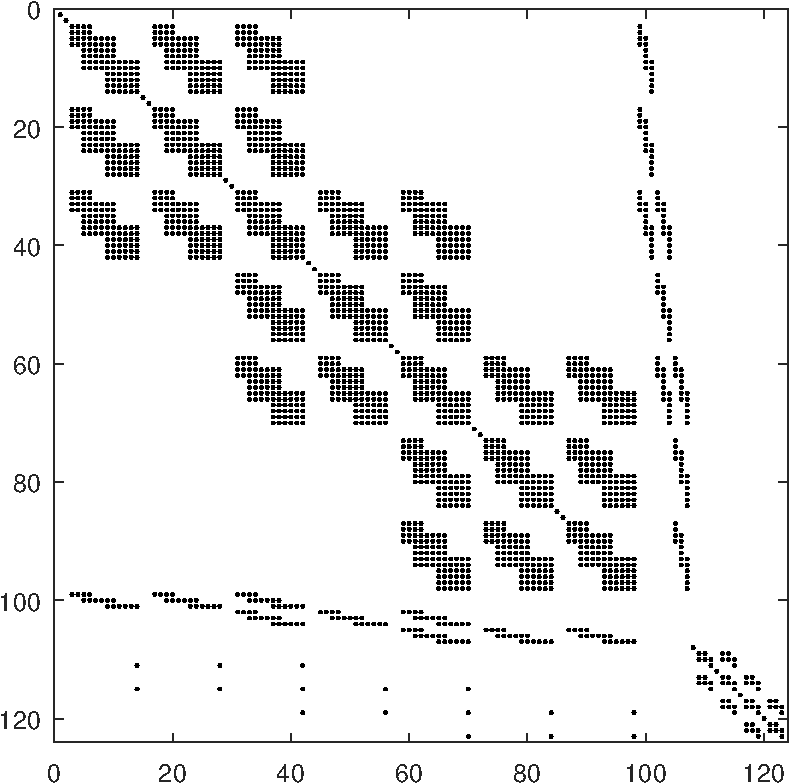
\includegraphics[width=0.6\textwidth]{figs/coarsespy.pdf}
\end{center}
\caption{FIXME block structure of coupled problem}
\label{fig:blockstructure}
\end{figure}


\section{Validation} \label{sec:validation}

FIXME


\section{Discussion and conclusion} \label{sec:discussion}

FIXME among many things cite \cite{LeysingerGudmundsson2004} regarding earlier comparison of stokes to Halfar

FIXME not appreciated that, while for explicit time-stepping schemes the surface mass balance need only be computed at the current ice surface, and at neighboring ice-free locations, in implicit time stepping the surface mass balance must be available to the evolving-geometry model (specifically to the residual-evaluation code) at every location in a 3D neighborhood of the ice surface, and indeed at all 3D locations above the bedrock elevation; a ``potential ice surface mass balance'' is needed at all such locations

\appendix
\section{The shallow ice approximation and its solutions}

The shallow ice approximation (SIA), a widely-used simplified model for the flow of grounded, non-sliding ice \cite{SchoofHewitt2013}, is applied in this paper only for comparison purposes.  It is derived by a small-parameter argument which we recall from Chapter 18 of \cite{Fowler1997}; similar arguments appear in other sources e.g.~\cite{GreveBlatter2009}.

Let $[H]$, $[L]$, $[U]$, and $[\tau]$ denote typical thickness, horizontal extent, horizontal velocity, and vertical-plane shear stress values, respectively, of a glacier.  We consider $\eps = [H]/[L]$ as the small parameter; for a mountain glacier we might have $\eps \approx 0.1$ but for the Greenland ice sheet $\eps \in (10^{-3},10^{-2})$ is reasonable.  We scale the kinematic variables $x,y \sim [L]$, $z \sim [H] = \eps [L]$, $u,v \sim [U]$, and $w \sim \eps [U]$.\footnote{Recall this means, for example, that we introduce new ``hatted'' variables via $x=[L]\hat x$, $y=[L]\hat y$, and $z=[H] \hat z$.  The equations are rewritten in the new variables and then the hats are removed.}  We suppose stress components $\tau_{xz},\tau_{yz}$ scale with $[\tau]$ and $\tau_{xx},\tau_{yy},\tau_{xy}$ with $\eps[\tau]$.   The pressure perturbation from the hydrostatic condition, namely $p-\rhoi g (h - z)$, is scaled with $\eps [\tau]$ also; this means that $p-\rhoi g (h - z)=\eps[\tau]\hat{\delta p}$.  With these scalings, plus certain additional relationships among the scale factors \cite{Fowler1997}, equation \eqref{forcebalance} yields
    $$\frac{\partial\tau_{xz}}{\partial z} + O(\eps^2) = \frac{\partial h}{\partial x}, \qquad \frac{\partial\tau_{yz}}{\partial z} + O(\eps^2) = \frac{\partial h}{\partial y}.$$
The shear strain rates are dominated by the $z$ derivatives of the horizontal velocity, thus
    $$\tau_{xz} = \nu\left(\frac{\partial u}{\partial z} + \eps^2 \frac{\partial w}{\partial z}\right), \qquad \tau_{yz} = \nu\left(\frac{\partial v}{\partial z} + \eps^2 \frac{\partial w}{\partial y}\right).$$
Also, the norm of the deviatoric stress satisfies $|\tau|^2 = \tau_{xz}^2 + \tau_{yz}^2 + O(\eps^2)$ and the stress-free condition at the surface $z=h$ becomes $\tau_{xz} = O(\eps^2)$ and $\tau_{yz} = O(\eps^2)$.  Note that incompressibility \eqref{incompressible} is unaltered by the scaling.

The strong form of the SIA arises from dropping terms of order $O(\eps^2)$ from the scaled equations and returning to the original, unscaled variables.  In order to compactly state these equations let $\bm{\tau}=\left<\tau_{xz},\tau_{yz}\right>$ denote the remaining shear stress components and $\bm{\omega}=\left<\frac{1}{2} \frac{\partial u}{\partial z},\frac{1}{2} \frac{\partial v}{\partial z}\right>$ the corresponding strain rates.  Note that \eqref{viscflowlaw} implies $|\bm{\tau}|=B_n |\bm{\omega}|^{1/n}$, where $|\cdot|$ denotes the ordinary Euclidean norm on $\RR^2$, and thus that $\bm{\omega} = A_n |\bm{\tau}|^{n-1} \bm{\tau}$ where $A_n=(B_n)^{-n}$.  We now have the following equations for the shear stresses and the velocity,
\begin{equation}
\frac{\partial\bm{\tau}}{\partial z} = \rhoi g \grad h, \qquad \Div \bu = 0, \qquad \bm{\omega} = A_n |\bm{\tau}|^{n-1} \bm{\tau}, \label{siavectorized}
\end{equation}
subject to $\bm{\tau}=0$ at the surface $z=h$ and $\bu=0$ on the base $z=b$.

The SIA stress equations \eqref{siavectorized} can be vertically-integrated to give a formulas for the horizontal velocity.  A first integral gives $\bm{\tau} = - \rhoi g (h-z) \grad h$, thus
    $$\left<\frac{\partial u}{\partial z},\frac{\partial v}{\partial z}\right> = - 2 A_n (\rhoi g)^n (h-z)^n |\grad h|^{n-1} \grad h.$$
Integrating again we determine the horizontal velocity at any point within the ice:
\begin{equation}
\left<u,v\right> = - \frac{2 A_n (\rhoi g)^n}{n+1} \left((h-b)^{n+1} - (h-z)^{n+1}\right) |\grad h|^{n-1} \grad h.  \label{siavelocity}
\end{equation}

The result in \eqref{siavelocity} is not actually our model for ice flow, but rather it has three ancillary purposes.  First, in combination with the hydrostatic pressure computation $p=\rhoi g (h-z)$, and vertical integration of the incompressibility equation to approximate $w$, it provides a fast computation of an initial iterate for a nonlinear Stokes solver.  Second, the computation of \eqref{siavelocity} on a given mesh defines our ``work unit'' when evaluating Stokes solver performance on that mesh.  Third, when combined with the surface kinematical equation, \eqref{siavelocity} can be used to derive a nonlinear and degenerate diffusion equation for the ice sheet thickness \cite{Fowler1997}.  We will use the following exact similarity solution of this diffusion equation as a source of synthetic ice sheet initial states in certain numerical experiments.

This solution arises from the $n=3$, flat-bed ($b=0$), and zero surface mass balance ($a=0$) case.  By integrating equation \eqref{siavelocity} vertically one may show that the scaled surface kinematical equation implies that the evolving ice thickness function $H(t,x,y)\ge 0$ solves
\begin{equation}
\frac{\partial H}{\partial t} = \Gamma \Div \left(H^5 |\grad H|^2 \grad H\right). \label{sia}
\end{equation}
on the set where $H>0$ \cite{Fowler1997}, where $\Gamma = \frac{2}{5} A_3 (\rhoi g)^3$.  References \cite{Bueler2016,Calvoetal2002,JouvetBueler2012} consider the rigorous meaning of this free boundary problem.  P.~Halfar \cite{Halfar1981} observed that \eqref{sia} has an exact similarity solution with $\lim_{t\to 0} H$ equal to a Dirac delta function, and that this solution is asymptotically stable.  In 3D \cite{Halfar1983} the solution is a circular dome which spreads radially while thinning, with constant-in-time total volume.  Denoting the radial coordinate as $r=(x^2+y^2)^{1/2}$, the solution is of the form $H(t,r) = t^{-\alpha} \varphi(s)$ with similarity variable $s=t^{-\beta} r$ and $\alpha=1/9$ and $\beta=1/18$.  If a center thickness $H_0$ and radius $R_0$ are given then, on the set where $H$ is positive \cite{Bueleretal2005},
\begin{equation}
H(t,x,y) = H_0 \left(\frac{t}{t_0}\right)^{-\alpha} \left\{1 - \left[\left(\frac{t}{t_0}\right)^{-\beta} \frac{r}{R_0}\right]^{4/3}\right\}^{3/7}. \label{halfar}
\end{equation}
The characteristic time is found by $t_0 = (\beta/\Gamma) (7/4)^3 R_0^4 H_0^{-7}$.  The corresponding 2D Halfar solution $H(t,x)$ \cite{Halfar1981}, in one horizontal dimension, is of the same form as \eqref{halfar} but with $r$ replaced by $x$ and with $\alpha=\beta=1/11$.

\small

\bigskip
\bibliography{simp}
\bibliographystyle{siam}

\end{document}
